%-----------------------------------------------------------------------------------------------
\documentclass[addpoints, 11pt]{exam}
\usepackage[margin=.75in]{geometry}
\usepackage{etex}
\usepackage{graphicx}
\usepackage{amssymb}
\usepackage[fleqn]{amsmath}
\usepackage{nccmath}
\usepackage{cases}
\usepackage{hyperref}
\usepackage{multicol}
\usepackage{enumerate}
\usepackage{tikz}
\usepackage{pgfplots}
\usetikzlibrary{patterns}
\usepackage{pstricks-add}
%\usepackage{pst-func}
%\usepackage{pst-plot}
%\usepackage{pst-spectra}
\usepackage{multido}
\usepackage{lastpage}
\usepackage{ulem}
\usepackage{float}
\usepackage[outside]{coordsys}
\usetikzlibrary{pgfplots.statistics}
\usetikzlibrary{positioning, shapes.geometric}
%-------------------------------------------------------------------------------------------------
\setlength{\columnsep}{.5cm}
\setlength{\columnseprule}{1pt}
\newcommand{\ds}{\displaystyle}
\newcommand{\work}{{\bf{No Work $\Leftrightarrow$ No Points }}}
\newcommand{\neat}{{\bf{Use Pencil Only $\Leftrightarrow$ Be Neat \& Organized }}}
\newcommand{\answer}{\large\bf Ans: \underline{\hspace{1.5in}}}
\newcommand{\la}{\lambda}
\newcommand{\zz}{\mathbb{Z}}
\newcommand{\rr}{\mathbb{R}}
\newcommand{\nn}{\mathbb{N}}
\newcommand{\qq}{\mathbb{Q}}
\newcommand{\cc}{\mathbb{C}}
\newcommand{\cyclic}[1]{\langle #1 \rangle}
\newcommand{\lcm}{{\rm{lcm}}}
\renewcommand{\solutiontitle}{\noindent\textbf{Answer:}\par\noindent}
%------------------------------------------------------------------------------------------------
\begin{document}
%------------------------------------------------------------------------------------------------
\cfoot{UCLA: C. Johnson}
%	\rfoot{Total Points: \numpoints}
\rfoot{Page \thepage\ of \pageref{LastPage}}
%------------------------------------------------------------------------------------------------
\begin{center}
\fbox{%
	\parbox{1\linewidth}{%
		\noindent \Large\bfseries \\[.05in] Math 142: Modeling{\hspace{1.2in}{\Large\bfseries Name:{\hrulefill}}\\[.2cm]
			\noindent \Large\bfseries Homework \# 4 \hspace{2.8in}{Due:} Friday Oct 27
		}\\[.025in]
	}%
}
\end{center}
\addpoints


\vspace{.25cm}


%------------------------------------------------------------------------------------------------
\noindent  {\bf Directions} Complete the exercises. Your solutions to the exercises should be submitted to Gradescope before the indicated due date above. Please follow rules regarding Gradescope submission as described in the syllabus. \\


\noindent{\bf References} Except for the help of the instructor or TAs and the class textbooks and notes, if you use any resources, for example, a book, a website, or you discussed with your friends, please acknowledge them in this References section. 
\begin{itemize}
\item I discussed Problem ?? with STUDENT A, STUDENT B, $\ldots$
\item I used BOOK/WEBSITE to help me do Problem ??.
\end{itemize}
\vspace{.05cm}
%\hrule
%----------------------------------------------------------------------------------------------  
\noindent {\bf Exercises}
%\begin{multicols*}{2}
\begin{questions}
%----------------------------------------------------------------------------------------------  
%----------------------------------------------------------------------------------------------  
\question 
\begin{parts}  
	\part Create a model of a pair of dice analogous to the coin model where there is an equal probability for each of the 6 numbers on each die. Run the model 100 times and make a graph of the resulting distribution. (Do NOT google for this code. Just tweak the coin model.) Plot the results.
	\begin{figure}[h!]
		\centering
		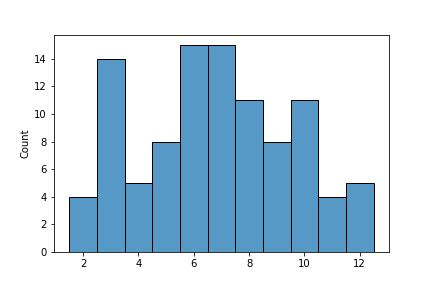
\includegraphics[scale=0.3]{die_unweighted.png}
	\end{figure}
	\part Create a second version where the dice are biased so that there is a $30\%$ greater chance of a six on each die. Plot the results.
	\begin{figure}[h!]
		\centering
		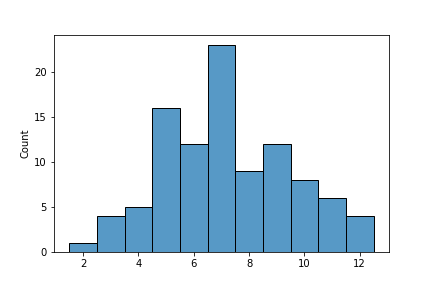
\includegraphics[scale=0.3]{die_weighted.png}
	\end{figure}
	\part Compare the two graphs and describe the results. 

	The top graph is more symmetric than the bottom graph because of a higher probability of a $6$s getting rolled in the bottom graph. The lower graph is slightly skewed to the left.
\end{parts}
%----------------------------------------------------------------------------------------------
%\question  {\bf Population genetics} We have argued that real populations have carrying capacities, at which rates of birth and death are equal. We can study the diversity of such populations (how many different cells will be present), using a Moran process model. Consider a population of $N$ cells, which we initially label $1,2,3, \ldots$. You task is to develop a simulation of how many descendants each of these starting cells has during the following process.\\
%
%In each unit of time, imagine that a randomly chosen cell among the $N$ divides. This produces another cell with the same label (so if a cell with label 2 divides, then the new cell also has label 2). But to keep the number of cells constant, a cell must die. Take another randomly chosen cell among the $N$ and remove it from the population. (It is possible that the same cell will divide and die in a single time step - that's ok).
%e.g. Suppose we start with 6 cells: $1,2,3, \ldots 6$ In our first step we find that cell 5 divides, and cell 2 dies. After the first step our cells are now labeled: $1,3,4,5,5,6$.
%\begin{parts}
%	\part Simulate 1000 time steps of this process using 6 cells. Show that after enough time steps all of the cells eventually have the same label (i.e. descend from only one of your starting cells).
%	\part Simulate 100 replicate populations, each with $N=6$ cells. Show that they all, eventually each
%	1
%	replicate population becomes homogeneous.
%	\part Explain: After 1000 time steps, what is the average number of descendants that cell number 1 should have among the 6 cells? Argue mathematically (hint: every cell should have the same average number of descendants), and then compare with the answer obtained from your numerical simulation.
%	\part The same homogenization occurs in populations of different sizes. Measure the average time taken for the population to become homogeneous in $N=3, N=10, N=15$ cells.
%	\part It has been argued that the average number of steps for the population to homogenize is proportional to $N^2$. Plot your data from (d) in a way that tests this relationship.
%	The process of homogenization is known as genetic drift, and is an important force in evolution. Although our model is for cells dividing, it also occurs in populations that reproduce sexually. In particular we inherit our mitochondrial DNA is inherited directly from our mothers. Through mitochrondial DNA it can be shown that we are each descendants of one of between 7 and 29 women (different genetic mapping methods produce different answers).
%\end{parts}
%----------------------------------------------------------------------------------------------   
\question {\bf Length of a polymer} Versions of the random walk model we created in class are used in polymer physics to model the sizes of polymers, such as strands of RNA. We imagine the polymer as a set of links, each of length 1. These links are arranged back and forth along a straight line (so the first link goes toward the left or right with equal probability, similarly the second, and we can simulate the configuration of a polymer with $N$ links as a $N$-step random walk).\\

A quantity of interest is how the maximum distance polymer gets from its starting position (0) if it has $N$ links. This distance is referred to as the radius of gyration of the polymer.
\begin{parts}
	\part Make a histogram of the observed radius of gyration of 100 polymers, each of which have 200 links. Notice that the histogram is not bell shaped.
	\begin{figure}[H]
		\centering
		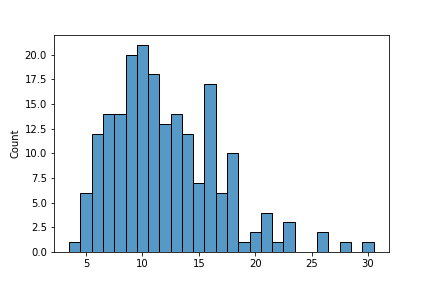
\includegraphics{100 polymers.png}
	\end{figure}
	\part It has been argued that the average radius of gyration is proportional to $\sqrt{N}$. By running 100 replicate simulations each with polymers of lengths $N=10,40,100,200$, and measuring the average radius of gyration for each length of polymer, test this theory.
	\begin{figure}[H]
		\centering
		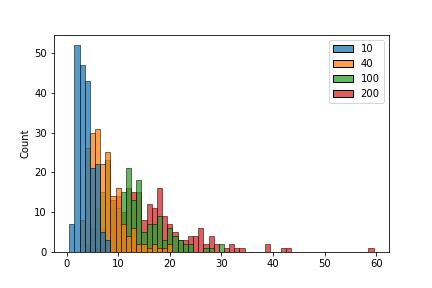
\includegraphics{10-200 polymers.png}
	\end{figure}
	The squares of our average lengths were $12.96,55.6516,151.5361,$ and $278.723025$ respectively. While these are somewhat similar to the number of lengths, $\sqrt{N}$ is probably an underestimate of the average length.
\end{parts}
Real polymers are arranged in 3D, but our model can describe how they may behave when confined (e.g. in virus).

%----------------------------------------------------------------------------------------------   
\question  In class we developed a mathematical model for stochastic population growth. Throughout this question, unless a question part instructs you to do otherwise, you may use the same parameters we adopted in class: $b=0.5$, $\Delta t=0.01$.
\begin{parts}
	\part Briefly describe in your own words, how we simulate numerically stochastic population growth.\\ 
	Our goal is to use randomness to predict the population size at a time step $t$. 
	Between each time step, every individual has the chance to reproduce (or die). 
	We use a random number generator to determine whether an individual is born/dies between censuses.
	We choose a time step small enough s.t the probability that the population changes by more than $1$ between time steps is insignificant. 
	Repeating the experiment several times, we can average the results from each experiment to determine the average population growth.
	\part In class we will explain why it is necessary to assume that $\Delta t$ is very small. Let's see why in your simulations. Plot on the same axes, graphs of the mean population size against time, among your 100 replicate simulations, when $\Delta t=0.01, \Delta t=0.1, \Delta t=1, \Delta t=2$. On the same plot draw the average population size that we predict theoretically: $N(t)=e^{b t}$. Comment on whether the simulations still follow theory for larger values of $\Delta t$.
	\begin{figure}[H]
		\centering
		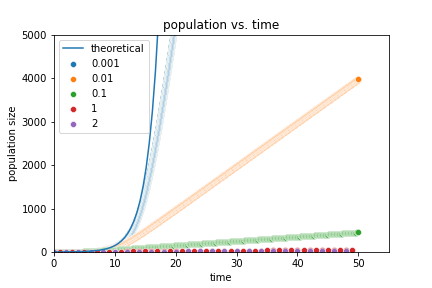
\includegraphics[scale=0.5]{stochastic_q_3_b.png}
	\end{figure}
	\part From the 100 replicate simulations, make a plot of the fraction of the simulations that have exactly two cells, as a function of time, $t$. On the same plot include the theoretical curve (which we will derive in class):
	$$
	P_2(t)=e^{-b t}\left(1-e^{-b t}\right) .
	$$
	\begin{figure}[H]
		\centering
		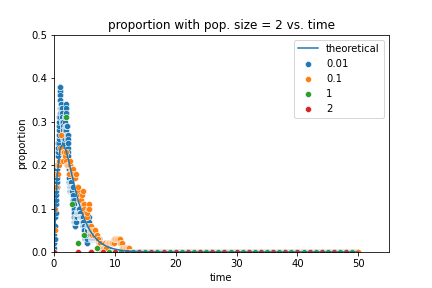
\includegraphics[scale=0.5]{stochastic_q_3_c.png}
	\end{figure}
	\part In our simulation we have neglected the effect of cell deaths. Now let's include this effect. In the code, after you have calculated the number of births (cells to add), consider the possibility that each cell that was present at time $t$ dies with probability $m \Delta t$. Assuming $m=0.2$, make a plot of the average population size as a function of time $t$, and compare with the deterministic result:
	$$
	N(t)=e^{(b-m) t} .
	$$
	Also answer: does every single one of your simulated populations grow exponentially?\\
	\begin{figure}[H]
		\centering
		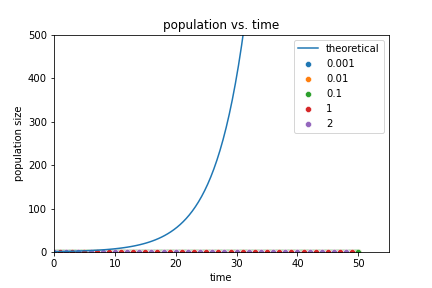
\includegraphics[scale=0.5]{stochastic_q_3_d.png}
	\end{figure}
	No. At low population levels $\approx1$ there is a high enough probability that the population could die entirely between the first censuses.
\end{parts}
%---------------------------------------------------------------------------------------------- 
\question We will build a stochastic model for how a population of bacteria is depleted by an antibiotic. Assume that at time $t=0$, there are precisely $N$ bacterial in the population. Once the antibiotic is added the bacteria stop dividing (that is $b=0$ ), and start to die with a mortality rate $m$. That is, in time $\Delta t$, the probability of a given cell dying is $m \Delta t$. We want to calculate the probability distribution, $P_n(t)$, which represents the probability that there are $n$ cells at time $t$.
\begin{parts}
	\part Explain what the initial conditions on $P_n(t)$ are.\\
	$P_n(0)=\begin{cases}
		1 & \text{for }n=N\\
		0 & \text{for }n\neq N
	\end{cases}$
	\part Show that
	$$
	\frac{d P_N}{d t}=-N m P_N
	$$
	and that:
	$$
	\frac{d P_n}{d t}=(n+1) m P_{n+1}-n m P_n
	$$
	for $n=0,1,2, \ldots N-1$.\\
	Notice that because $b=0$, the population is at most $N$.\\
	$\displaystyle P_n(t+\Delta t)=\sum_{k=n}^{N}\begin{pmatrix}
		k\\
		k-n
	\end{pmatrix}(m\Delta t )^{k-n} (1-m\Delta t )^{n}P_k(t)$\\
	$\displaystyle\frac{P_n(t+\Delta t)-P_n(t)}{\Delta t} =\frac{\sum_{k=n}^{N}\begin{pmatrix}
		k\\
		k-n
	\end{pmatrix}(m\Delta t )^{k-n} (1-m\Delta t )^{n}P_k(t)}{\Delta t}-\frac{P_n(t)}{\Delta t}$\\
	$\frac{dP_n(t)}{dt}=\lim_{\Delta t\rightarrow 0}\frac{P_n(t+\Delta t)-P_n(t)}{\Delta t}=\lim_{\Delta t\rightarrow0}\frac{({(1-m\Delta t)}^n-1)P_n(t)}{\Delta t}+\frac{(n+1)m\Delta t({(1-m\Delta t)}^n)P_{n+1}(t)}{\Delta t}+O(\Delta t)$\\
	$=\lim_{\Delta t\rightarrow0}\frac{(1-nm\Delta t-1)P_n(t)+O(\Delta t)}{\Delta t}+\frac{(n+1)m\Delta t P_{n+1}(t)+O(\Delta t)}{\Delta t}$\\
	$=(n+1)mP_{n+1}(t)-nmP_n(t)$ where $P_{N+1}(t)=0$ for all $t$.
	\part Solve the first few differential equation to calculate $P_N(t), P_{N-1}(t)$ and $P_{N-2}(t)$. Can you see any pattern that would help you to guess $P_n(t)$ (reading Chapter 36 in the book might help you with this). You do not need to prove that your answer is correct.\\
	$P_N(t)=e^{-mNt}$\\
	$\frac{dP_{N-1}}{dt}+(N-1)mP_{N-1}(t)=Nme^{-Nmt}\Rightarrow (e^{(N-1)t}P_{N-1}(t))'=Nme^{-mt}\\
	\Rightarrow e^{(N-1)t}P_{N-1}(t)=-Ne^{-mt}+c$ Applying initial condition $P_{N-1}(0)=0$ we obtain $P_{N-1}(t)=Ne^{-(N-1)mt}(1-e^{-mt})$\\
	$\frac{dP_{N-2}}{dt}+(N-2)mP_{N-2}(t)=N(N-1)me^{-(N-1)mt}(1-e^{-mt})\\
	\Rightarrow (e^{(N-2)t}P_{N-2}(t))'=N(N-1)me^{-mt}(1-e^{-mt})\\
	\Rightarrow e^{(N-2)t}P_{N-2}(t)=\frac{N(N-1)}{2}{(1-e^{-mt})}^2+c$ Applying initial condition $P_{N-2}(0)=0$ we obtain $P_{N-2}(t)=\frac{N(N-1)}{2}e^{-(N-2)mt}{(1-e^{-mt})}^2$\\
	$P_n(t)=\begin{pmatrix}
		N\\
		N-n
	\end{pmatrix}e^{-nmt}{(1-e^{-mt})}^{N-n}$ 
	\part Verify that your solution for $P_N(t)$ is correct, by comparing it with stochastic simulations. Specifically, implement a stochastic simulation for the death of bacteria (you are free to decide for yourself how many replicates you want to run). For sake of definiteness, run the simulations with $0<t<10$, and $m=1.2$, and $N=15$. 
	\begin{figure}[H]
		\centering
		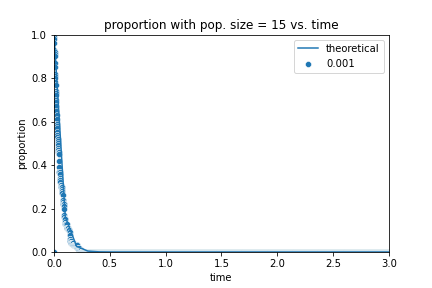
\includegraphics[scale=0.5]{stochastic_q_4_d.png}
	\end{figure}
	\part It is hard to see how, on average, the population will change over time, using the formulas for the $P_n(t)$. But we can get this average directly. Suppose that at time $t$, the average number of cells in the population is $\bar{n}(t)$. Between time $t$ and $t+\Delta t$, how many cells, on average, will die? Use this information to derive a differential equation:
	$$
	\frac{d \bar{n}}{d t}=-m \bar{n} .
	$$
	$\bar{n}(t)=\sum_{n=0}^{N}nP_n(t)=Ne^{-mt}$ by average of binomial dist. $\lim_{\Delta t\rightarrow 0}\frac{Ne^{-m(t+\Delta t)}-Ne^{-mt}}{\Delta t}=-Nme^{-mt}\Rightarrow\frac{d\bar{n}(t)}{dt}=-m\bar{n}(t)$
	\part Solve the differential equation from part (e) and show that it agrees with the average population size according to stochastic numerical simulations. Use the same parameter values as in part (d).
	\begin{figure}[H]
		\centering
		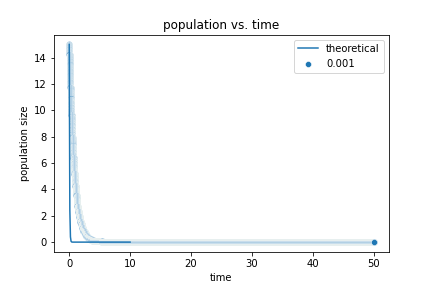
\includegraphics[scale=0.5]{stochastic_q_4_f.png}
	\end{figure}
\end{parts}
%----------------------------------------------------------------------------------------------
\question We are building a model for how a material like concrete degrades due to cracks forming. Let's assume that in a time interval $\Delta t$ there is a probability $f \Delta t$ of a new crack forming (we call $f$ the fracture rate). Assume moreover that at time $t=0$ there are no cracks in the material. Let $P_n(t)$ be the probability that there are exactly $n$ cracks in the material at time $t$.
\begin{parts}
	\part Show that:
	$$
	\frac{d P_n}{d t}=f P_{n-1}-f P_n \quad, \quad \text { if } n>0
	$$
	and derive the differential equation for $P_0(t)$. what are the initial conditions for all of your differential equations?
	$P_n(t)=\begin{cases}
		1 & \text{ for }n=0\\
		0 & \text{ for }n\neq0
	\end{cases}$\\
	$P_{n}(t+\Delta t)=f\Delta t P_{n-1}(t)+(1-f\Delta t)P_{n}(t)\Rightarrow \frac{P_{n}(t+\Delta t)-P_{n}(t)}{\Delta t}=fP_{n-1}(t)-fP_{n}(t)$. Taking the limit as $\Delta t$ goes to $0$ we obtain $\frac{d P_n}{d t}=f P_{n-1}-f P_n$, and because $P_{-1}(t)=0$ for all $t$, $\frac{d P_0}{d t}=-f P_0$
	\part Find a differential equation describing the average number of cracks in each replicate sample.
	Let $\bar{n}(t)$ be the average number of cracks at time $t$. $\bar{n}(t+\Delta t)-\bar{n}(t)=(1+f\Delta t)\bar{n}(t)-\bar{n}(t)\Rightarrow\frac{d\bar{n}(t)}{dt}=f\Rightarrow \bar{n}(t)=e^{ft}-1$
	\part We have to replace the concrete when it reaches 10 cracks. Assume that $f=1$. Using stochastic simulations, make a histogram based on 100 replicate simulations, representing 100 samples of the concrete, showing the range of times at which each sample had to be replaced (i.e. reached 10 cracks).
\end{parts}
%----------------------------------------------------------------------------------------------
\question Submit the code you used for any and all of the problems. (Print pdf the code) Either lump it all together at the end or when matching problems on Gradescope, select all pages of pdf that has code if you included code within the solution to each answer.
%----------------------------------------------------------------------------------------------
\end{questions}
%\end{multicols*}
\end{document}